\documentclass{report}
% Comment the following line to NOT allow the usage of umlauts
\usepackage[utf8]{inputenc}
\usepackage[francais]{babel}
\usepackage{listings}
\usepackage{xcolor}
\usepackage{textcomp}
\usepackage{graphicx}
\usepackage{hyperref}
\pagestyle{plain}
\definecolor{listinggray}{gray}{0.9}
\definecolor{lbcolor}{rgb}{0.9,0.9,0.9}
\lstset{
 backgroundcolor=\color{lbcolor},
 tabsize=4,
 rulecolor=,
 language=matlab,
 basicstyle=\scriptsize,
 upquote=true,
 aboveskip={1.5\baselineskip},
 columns=fixed,
 showstringspaces=false,
 extendedchars=true,
 breaklines=true,
 prebreak = \raisebox{0ex}[0ex][0ex]{\ensuremath{\hookleftarrow}},
 frame=single,
 showtabs=false,
 showspaces=false,
 showstringspaces=false,
 identifierstyle=\ttfamily,
 keywordstyle=\color[rgb]{0,0,1},
 commentstyle=\color[rgb]{0.133,0.545,0.133},
 stringstyle=\color[rgb]{0.627,0.126,0.941},
}
% Start the document
\begin{document}
\begin{titlepage}
  \begin{sffamily}
  \begin{center}

    \huge \textsc{Manuel utilisateur de WarBot}\\[5cm]
  \end{center}

  \end{sffamily}
\end{titlepage}
  
\tableofcontents
\newpage
%%%
% PARTIE Interface Graphique
%%%
\chapter{Partie Interface Graphique}
\section{Présentation}
La partie Interface Graphique comprend principalement l'habillage visuel des éléments avec lequel l'utilisateur va interagir pour jouer au jeu. MetaBot étant un jeu pour "programmeur", le joueur interagi surtout avec le menu principal et l'éditeur de comportement afin de créer des équipes pour pouvoir les faire s'affronter.
\paragraph{}
L'interface graphique que nous avons créé se décompose en quatre parties, le menu principal, le menu de paramètre, l'éditeur de comportement et des fonctionnalités directement en jeu.
\paragraph{}
Le premier choix a donc été de revoir totalement l'interface, ce que nous pouvions faire grâce aux nouveaux éléments apportés. En effet il fallait rajouter de nouvelles fonctionnalités basiques à cette interface qui en avait finalement très peu et ajouter un peu de couleurs à tout ça.


\section{Menu Principal}
\paragraph{}
Voici l’écran de menu principal. Ceci est le premier écran qui apparaîtra lorsque vous lancerez le jeu.
Passons en revue toutes les possibilités que ce menu offre.
\subsection{Lancer une Partie}
En cliquant sur ce bouton, la partie se lancera, et le combat pourra commencer !

\begin{figure}[!h]
	\centering
		
\includegraphics[scale=0.65]{BoutonJouer}
	\caption{Bouton Jouer}
\end{figure}
\subsection{Bouton Editeur de Comportement}
Ce bouton vous mènera à l’éditeur de comportement, pour gérer le comportement des unités de vos équipes.

\begin{figure}[!h]
	\centering
		
\includegraphics[scale=0.80]{Bouton_Editer}
	\caption{Bouton Éditer}
\end{figure}
\subsection{Bouton Paramètre}
Voici le menu paramètres, qui offre plusieurs choix de personnalisations.

\begin{figure}[!h]
	\centering
		
\includegraphics[scale=0.80]{Bouton_Parametre}
	\caption{Bouton Paramètre}
\end{figure}
\subsection{Choisir le nombre d'équipe}
Permet de choisir le nombre de joueurs. 2 joueurs minimum, 4 maximum.

\begin{figure}[!h]
	\centering
		
\includegraphics[scale=0.60]{Selection_nb_joueurs}
	\caption{Sélection du nombre de joueur}
\end{figure}
\subsection{Choisir les équipes}
Choix des équipes pour chaque joueur.

\begin{figure}[!h]
	\centering
		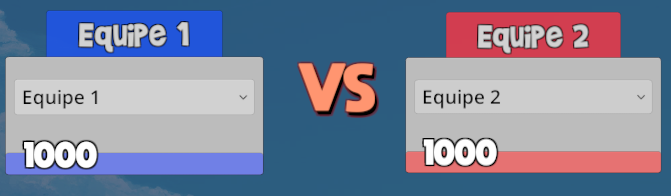
\includegraphics[scale=0.60]{Selection_Equipes}
	\caption{Sélection de l'équipe}
\end{figure}
\subsection{Bouton "Reload Team"}
Ce bouton permet de recharger les équipes.
\subsection{Bouton pour quitter le jeu}
Ce bouton ouvre une boite de dialogue demandant à l'utilisateur si il veut vraiment quitter le jeu. Il peut ainsi choisir de revenir sur le menu principal ou de fermer le jeu.
\subsection{Choisir carte de jeu}
Vous permet de choisir entre plusieurs cartes de jeu.

\begin{figure}[!h]
	\centering
		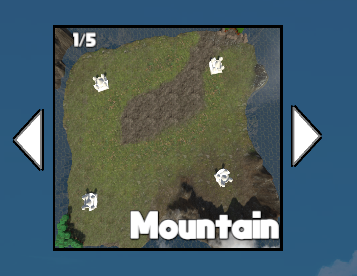
\includegraphics[scale=0.80]{Selection_Map}
	\caption{Sélection de la carte de jeu}
\end{figure}
\subsection{Choisir nombre de départ de chaque unités}
Détermine, pour chaque unité, le nombre avec lequel vous commencerez la partie.

\begin{figure}[!h]
	\centering
		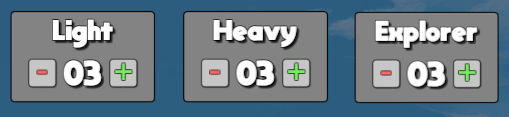
\includegraphics[scale=0.80]{Nombre_Unit}
	\caption{Choix du nombre d'unités}
\end{figure}


\subsection{Paramètres}
Voici le menu paramètres, qui offre plusieurs choix de personnalisations.
\begin{figure}[!h]
	\centering
		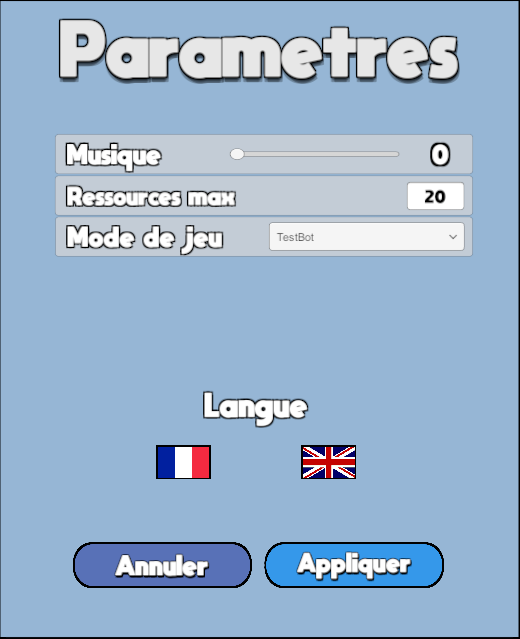
\includegraphics[scale=0.50]{Ecran_Parametre}
	\caption{Écran Paramètres}
\end{figure}


\subsection{Changer le Volume de la musique}
Permet de régler le volume du jeu
\begin{figure}[!h]
	\centering
		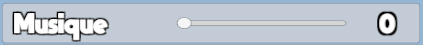
\includegraphics[scale=0.80]{Control_Musique}
	\caption{Volume de la musique}
\end{figure}


\subsection{Choisir nombre de ressource maximum dans le jeu}
Cette option vous permet de définir le nombre maximal de ressources présentes au même moment sur le sol
\begin{figure}[!h]
	\centering
		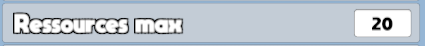
\includegraphics[scale=0.80]{Limite_Ressources}
	\caption{Nombre de ressource maximum}
\end{figure}


\subsection{Choisir le mode de jeu}
Vous pouvez sélectionner le mode de jeu que vous désirez.
\subsubsection{TestBot}
Le mode par défaut.
\begin{figure}[!h]
	\centering
		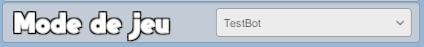
\includegraphics[scale=0.80]{ModeJeuTestBot}
	\caption{Choix du mode de jeu}
\end{figure}


\subsubsection{RessourceRace}
Deux nouvelles options apparaissent sous ce mode :
\begin{figure}[!h]
	\centering
		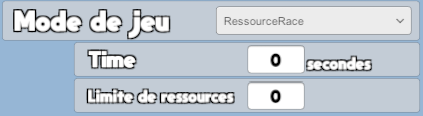
\includegraphics[scale=0.80]{ModeJeuRessourceRace}
	\caption{Options du mode RessourceRace}
\end{figure}

Temps: \newline
Vous permet de choisir la durée maximale d’une partie/\newline

Limite de ressources:\newline
La condition de victoire. La première équipe à avoir atteint cette limite remporte la partie

\subsection{Choisir la langue}
Choisissez la langue que vous préférez, simplement en cliquant sur le drapeau correspondant.
\begin{figure}[!h]
	\centering
		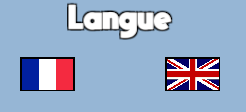
\includegraphics[scale=0.80]{Choix_Langue}
	\caption{Choix de la langue}
\end{figure}


\subsection{Bouton Retour}
Ce bouton annule tous les changements qui ont pu être fait, et vous renvoie au menu principal
\subsection{Bouton Valider}
Ce bouton valide les paramètres, puis vous renvoie au menu principal.
\begin{figure}[!h]
	\centering
		
\includegraphics[scale=0.80]{ApplyCancelSettings}
	\caption{Annuler ou Appliquer les changements}
\end{figure}
\clearpage






\section{Editeur de Comportement}
Cet écran vous permet d’éditer le comportement des unités de vos équipes.
\begin{figure}[!h]
	\centering
		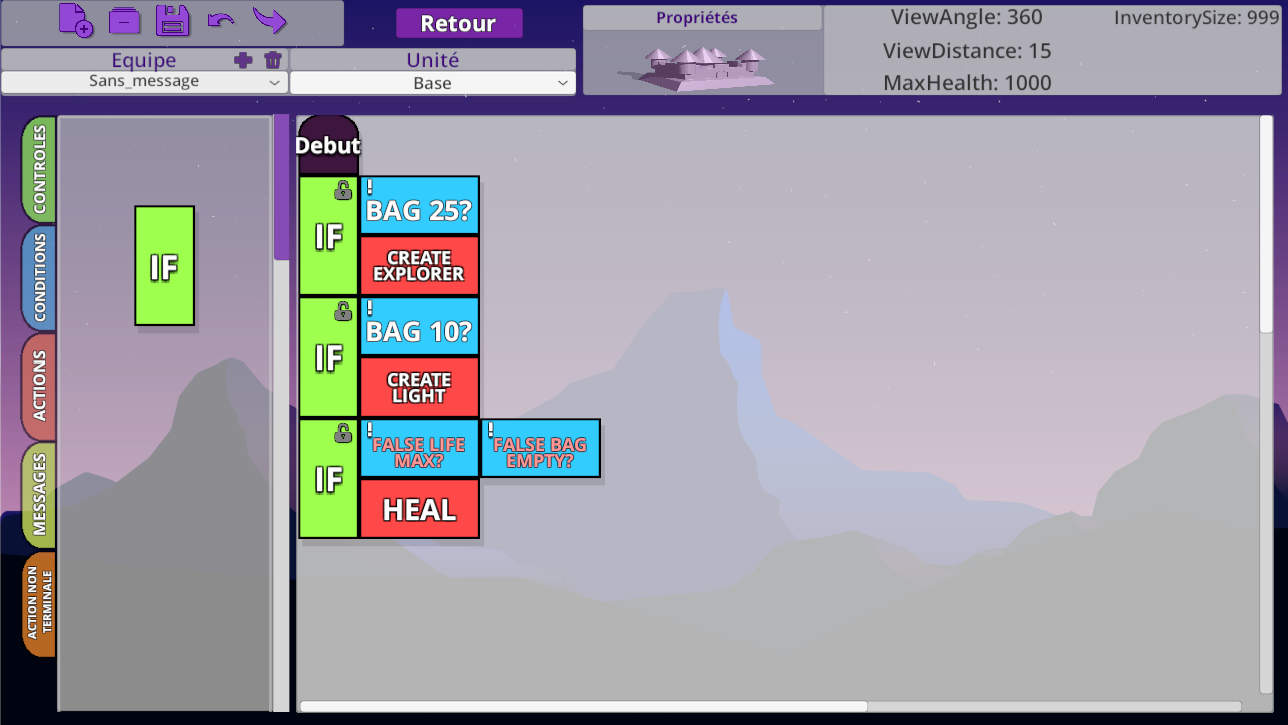
\includegraphics[scale=0.35]{Ecran_Editeur}
	\caption{Écran de l'éditeur}
\end{figure}
% ToolBox %

\subsection{Bouton Nouveau Comportement}
Ce bouton vous permet d’ouvrir un nouveau comportement vide, écrasant le comportement actuellement traité
\subsection{Bouton Chargement Comportement}
Permet de charger le comportement de l’unité active
\subsection{Bouton Sauvegarde du Comportement}
Permet de sauvegarder le comportement de l’unité en cours d’édition
\subsection{Bouton "Undo"}
Permet d’annuler la dernière création ou suppression de pièce
\subsection{Bouton "Redo"}
Permet de restituer la dernière annulation
\subsection{Bouton de retour au menu principal}
Renvoie au menu principal
% IMAGE TOOLBOX
\begin{figure}[!h]
	\centering
		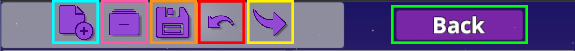
\includegraphics[scale=0.80]{ToolBoxSelectedArea}
	\caption{Boutons de la ToolBox}
\end{figure}

% Equipe + Unité %
\subsection{Choix de l'équipe}
Ce menu déroulant vous permet de choisir l’équipe sur laquelle travailler.
\subsection{Choix de l'unité}
Permet de créer une nouvelle équipe.
% IMAGE TEAM + UNIT
\begin{figure}[!h]
	\centering
		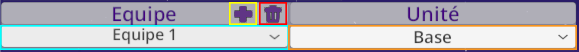
\includegraphics[scale=0.80]{Team_UnitSelectedArea}
	\caption{Sélection équipe et unité}
\end{figure}


\subsection{Bouton Création d'équipe}
Permet de créer une nouvelle équipe.
\subsection{Bouton Suppression d'équipe}
Permet de supprimer l’équipe actuellement sélectionnée.
\subsection{Affichage du modèle 3D de l'unité courante}
La zone en violet représente le modèle de l'unité actuellement sélectionnée.
\subsection{Affichage des statistiques de l'unité courante}
La zone en bleu affiche ses statistiques.
%IMAGE STATS + MODEL
\begin{figure}[!h]
	\centering
		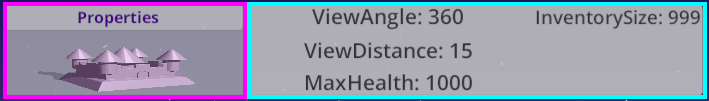
\includegraphics[scale=0.60]{StatsModeleUnitSelectedAreas}
	\caption{Statistiques et modèle de l'unité}
\end{figure}


% Zone de création des comportements
\subsection{Pièces de comportement}


\begin{minipage}{0.4\linewidth}
\paragraph{}
Ici se trouve la totalité des pièces à votre disposition pour la création de comportements.
Les pièces sont classées par type.
\end{minipage}
\begin{minipage}{0.2\linewidth}
\
\end{minipage}
\begin{minipage}{0.4\linewidth}
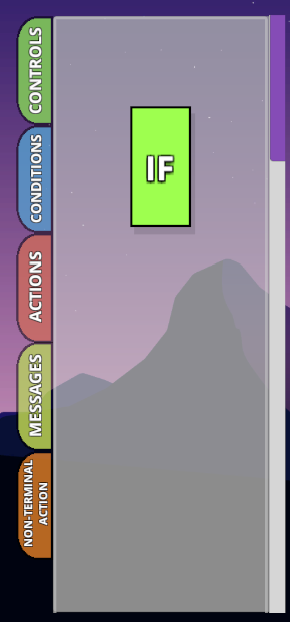
\includegraphics[scale=0.40]{Pieces}
\end{minipage}\hfill





\subsection{Zone d'édition}
Zone de création et d’édition de comportement.
\begin{figure}[!h]
	\centering
		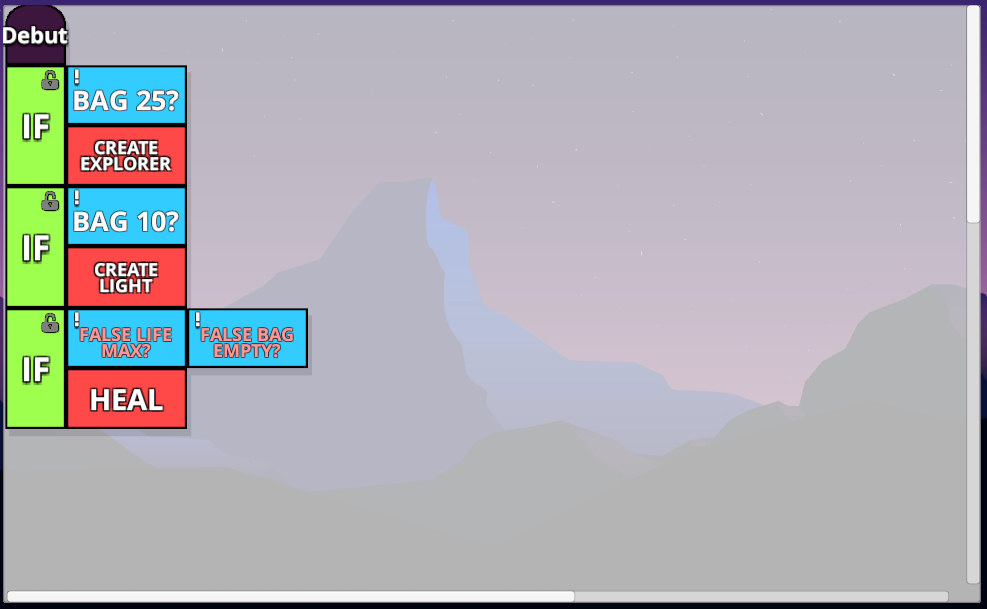
\includegraphics[scale=0.40]{Editeur}
	\caption{Éditeur de comportement}
\end{figure}


\section{Element dans le jeu}
\subsection{Réglage du volume du son}
Permet de régler le son durant une partie.
\begin{figure}[!h]
	\centering
		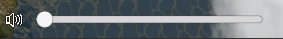
\includegraphics[scale=0.80]{SoundIG}
	\caption{Volume du son en jeu}
\end{figure}

\subsection{Outil de debug}
Cliquer sur ces boutons permet d'activer ou désactiver l'affichage de certaines informations.
\begin{figure}[!h]
	\centering
		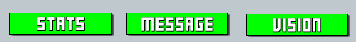
\includegraphics[scale=0.80]{sebug.png}
	\caption{Outils de debug}
\end{figure}
\paragraph{}
Cliquer sur le bouton "Stats" affecte l'affichage des barres de vie et du nombre de ressources de l'unité. \newline
Cliquer sur le bouton "Message" affecte l'affichage des traits entre les unités qui représentent les envois de message entre ces dernières. \newline
Cliquer sur le bouton "Vision" affecte l'affichage des cône de vision des unités.

\subsection{Caméras}
Cliquer sur ces boutons permet de changer de caméra.
\begin{figure}[!h]
	\centering
		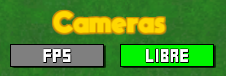
\includegraphics[scale=0.80]{camera.png}
	\caption{Caméras}
\end{figure}
\paragraph{}
Pour activer la vue à la première personne, il faut cliquer sur une unité. La caméra suit les mouvements de l'unit sur laquelle on a cliqué. Bouger la souris à droite ou à gauche modifie l'orientation de la caméra. Cliquer sur le bouton "FPS" permet de retourner en vue de dessus. \newline
Cliquer sur le bouton "Libre" permet d'activer ou désactiver la caméra libre. En mode caméra libre, il possible de modifier la position de la caméra en emmenant la souris sur les bords de la fenêtre. Il est également possible de zoomer. Si la caméra n'est pas libre, elle changera elle même sa position pour capturer au mieux l'entièreté des unités.

\subsection{Vitesse}
Modifier ce slider modifie la vitesse du jeu. 100\% représente la vitesse normale. Si la valeur est inférieur à 100\%, le jeu est ralentit. Si la valeur est au-dessus de 100\%, le jeu est accéléré. \newline
Il est possible d'appuyer sur espace pour passer la vitesse à 0\% automatiquement, ce qui met le jeu en pause.
\begin{figure}[!h]
	\centering
		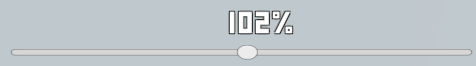
\includegraphics[scale=0.80]{vitesse.png}
	\caption{Changement de vitesse}
\end{figure}

\subsection{Boutons}
\begin{figure}[!h]
	\centering
		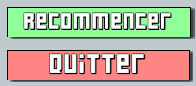
\includegraphics[scale=0.80]{quitter.png}
	\caption{Boutons quitter recommencer}
\end{figure}
\paragraph{}
Cliquer sur le bouton "Quitter" permet de revenir à l'écran principal, ce qui arrête la partie. \newline
Cliquer sur le bouton "Recommencer" permet de lancer une nouvelle partie avec les mêmes paramètres qui ont permis de lancer la partie en cours.

\chapter{Documentation primitives}
\section{Explication}
\paragraph{}
Les primitives permettent de modifier le comportement d'un certain type d'unité au sein d'une même équipe. Pour créer une primitive, il faut cliquer sur l'un des blocs dans le menu de gauche. Une primitive est alors positionné dans l'éditeur de comportement. \newline
Pour changer le type de primitives à créer, il faut cliquer sur les onglets de couleurs tout à droite de la fenêtre. \newline
Il faut ensuite la déplacer au bon endroit pour qu'elle soit prise en compte dans le comportement. Pour cela, il suffit de cliquer avec le clic gauche de la souris sur la primitive, de maintenir le bouton enfoncé et de déplacer sa souris. \newline
Il est possible de supprimer une primitive en faisant un clic droit sur l'une de celles dans l'éditeur de comportement.\newline
Une fois le comportement d'une unité terminé, il faut cliquer sur le bouton de sauvegarde pour que les unités de votre équipe puissent le suivre. \newline
Il est possible d'annuler la suppression ou la création d'une primitive en cliquant sur le bouton retour arrière.  \newline
Le bouton rétablir permet d'annuler les dernières modifications faites avec le bouton retour arrière.
\section{Start}
La primitive start est une primitive placé automatiquement dans chaque comportement. Elle est impossible à supprimer. Il n'existe aucun moyen d'en créer une seconde dans un même comportement. Pour qu'une primitive soit compté dans le comportement, il faut qu'elle soit reliée à la primitive start.
 \begin{figure}[!h]
	\centering
		
\includegraphics[scale=1]{start.png}
	\caption{Primitive start}
\end{figure}
\section{Controles}
La seule primitive de contrôle est "If". Elle est essentielle à la construction de comportement car c'est la seul primitive pouvant se déplacer en dessous de la primitive Start.\newline
Les If se placent les un en-dessous des autres. La partie haute du bloc est destiné aux conditions et la partie basse aux actions et messages.
\begin{figure}[!h]
	\centering
		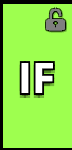
\includegraphics[scale=1]{if.png}
	\caption{Primitive de contrôle}
\end{figure}
\paragraph{}
\newpage
\section{Conditions}
\paragraph{}
Les conditions se placent sur la partie haute d'un if ou à droite d'une autre condition. Elles permettent d'exécuter les actions placées sur la partie basse du if si toutes les conditions sont vérifiés.
\begin{figure}[!h]
	\centering
		
\includegraphics[scale=1]{cond.png}
	\caption{Primitive de condition}
\end{figure}
\paragraph{}
\subsection{Conditions communes}
La liste des conditions communes à chaque unité est :
\begin{itemize}
\item Message à l'aide : vérifie si l'unité à reçut un message Demander de l'aide
\item Message position : vérifie si l'unité à reçut un message Donner sa position
\item Message attaquer : vérifie si l'unité à reçut un message Ordonner l'attaque
\item Message position ressource : vérifie si l'unité à reçut un message Donner position de ressource
\item Vie au niveau max : Vérifie si la vie actuelle de l'unité est égale à  sa vie maximale
\item Vie \textgreater 75\% : Vérifie si la vie actuelle de l'unité est supérieur à  75\% de sa vie maximale
\item Vie \textgreater 50\% : Vérifie si la vie actuelle de l'unité est supérieur à  50\% de sa vie maximale
\item Vie \textgreater 25\% : Vérifie si la vie actuelle de l'unité est supérieur à  25\% de sa vie maximale
\item Sac plein : Vérifie si le le nombre de ressource de l'unité est égale à la taille de son inventaire
\item Sac vide : Vérifie si l'unité n'a pas de ressources sur elle.
\item \textgreater 10 ressources dans sac : Vérifie si l'unité a au moins 10 ressources dans son sac
\item \textgreater 25 ressources dans sac : Vérifie si l'unité a au moins 25 ressources dans son sac
\item Ennemi à portée : Vérifie si un ennemi est dans le champ de vision de l'unité. Modifie la cible de l'unité
\item Allié à portée : Vérifie si un allié est dans le champ de vision de l'unité. Modifie la cible de l'unité
\end{itemize}
\subsection{Conditions explorer, light, heavy}
La liste des conditions communes aux explorer, light et heavy est :
\begin{itemize}
\item Est bloqué : vérifie si l'unité ne peux pas avancer à cause d'un obstacle
\item Base alliée Proche : Vérifie si une base alliée est dans le champ de vision de l'unité. Modifie la cible de l'unité
\item Can give : vérifie si l'unité peut donner une ressource à une autre unité
\item Contract Elimination : vérifie si l'unité a un contrat d'élimination en cours
\item Contract Elimination target near : Vérifie si la cible du contrat de l'unité est dans son champs de vision
\item Nourriture proche : Vérifie si une ressource est suffisamment proche pour être récupérée par l'unité
\item A un contrat : 
\item Nourriture a portée : Vérifie si une ressource est dans le champ de vision de l'unité
\end{itemize}
\subsection{Conditions ligh, heavy}
Il reste une condition commune aux light et aux heavy : \newline
Est recharge : Vérifie si l'unité est rechargé
\section{Acions}
\paragraph{}
Les actions permettent de faire agir les unités. Les actions se placent sur la partie basses d'un if et ne sont exécutés que si toutes les conditions placés dans la partie haute du if sont validés. Les actions terminent le tour de l'unité.
\begin{figure}[!h]
	\centering
		
\includegraphics[scale=1]{action.png}
	\caption{Primitive d'action}
\end{figure}
\paragraph{}
\subsection{Actions communes}
La liste des actions communes à chaque unité est :
\begin{itemize}
\item Ne rien faire : Termine le tour de l'unité
\item Donner une ressource : Donne une ressource à la cible de l'unité
\item Se soigner : Consomme une ressource pour récupérer de la vie
\end{itemize}
\subsection{Actions explorer, light, heavy}
La liste des actions communes aux explorer, light et heavy est :
\begin{itemize}
\item Avancer orientation aléatoire : modifie l'orientation de l'unité et la fait avancer d'un pas.
\item Se retourner puis avancer : L'unité se retourner puis avance d'un pas
\item Rentrer à la base : L'unité se tourne vers la base et avance d'un pas
\item Ramasser : L'unité ramasse une des ressource à sa porté
\end{itemize}
\subsection{Actions light, heavy}
La liste des actions communes aux light et heavy est :
\begin{itemize}
\item Tirer : lance un projectile droit devant soit
\item Recharger : L'unité recharge son arme
\end{itemize}
\subsection{Actions bases}
La liste des actions spécifiques aux base est :
\begin{itemize}
\item Créer Explorer (sac) : Crée une unité de type Explorer à l'aide des ressources de la base
\item Créer Light (sac) : Crée une unité de type Light à l'aide des ressources de la base
\item Créer Heavy (sac) : Crée une unité de type Heavy à l'aide des ressources de la base
\item Créer Explorer (vie) : Crée une unité de type Explorer en utilisant la vie de la base
\item Créer Light (vie) : Crée une unité de type Light en utilisant la vie de la base
\item Créer Heavy (vie) : Crée une unité de type Heavy en utilisant la vie de la base
\item Recharger : L'unité recharge son arme
\end{itemize}
\newpage
\section{Messages}
\paragraph{}
Les messages permettent de communiquer avec les unités spécifiés via un paramètre géré par un menu déroulant. Ils se placent sur la partie basse d'un if ou à droite d'un autre message ou d'une action non terminale. Le message n'est envoyé que si les conditions du if sont toutes validées. Les messages ne terminent pas le tour de l'unité\newline
\begin{figure}[!h]
	\centering
		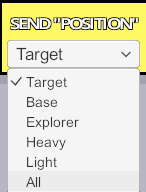
\includegraphics[scale=1]{msg.png}
	\caption{Primitive de message}
\end{figure}
\paragraph{}
La liste des messages communs à chaque unité est :
\begin{itemize}
\item Demander de l'aide : Envoit un message de type aide aux unités spécifiés dans le menu déroulant
\item Donner se position : Envoit un message de type position aux unités spécifiés dans le menu déroulant
\item Ordonner attaque : Envoit un message de type attaque aux unités spécifiés dans le menu déroulant
\item Donner la position de ressource : Envoit un message de type position ressources aux unités spécifiés dans le menu déroulant
\end{itemize}
\newpage
\section{Actions non terminale}
\paragraph{}
Les actions non terminales permettent de faire agir l'unité. Elles se placent sur la partie basse d'un if ou à droite d'une autre action non terminale ou d'un message. L'action n'est effectué que si les conditions du if sont toutes validées. Les actions non terminales ne terminent pas le tour de l'unité.
\begin{figure}[!h]
	\centering
		
\includegraphics[scale=1]{action2.png}
	\caption{Primitive d'ation non terminale}
\end{figure}
\paragraph{}
La liste des actions non terminales communes à chaque unité est :
\begin{itemize}
\item Se tourner au sud : Se tourne vers le bas de la fenêtre
\item Se tourner au nord : Se tourne vers le haut de la fenêtre
\item Se tourner à l'est: Se tourne vers la droite de la fenêtre
\item Se tourner à l'ouest : Se tourne vers la gauche de la fenêtre
\item Se tourner aléatoirement : Prend une orientation aléatoire
\item Se retourner : Fait un demi tour sur elle-même
\item Se tourner vers l'expéditeur: Se tourne vers l'expéditeur du dernier message perçu
\item Ajouter contrat d'élimination : Crée un ontrat d'élimination à partir de la cible actuelle de l'unité
\end{itemize}
\end{document}
